\section{Results}
\label{sec:Results}
% Chaos
From figure \ref{fig:Contour} (see also figure \ref{fig:AllProbabilities} in the Online Appendix) we conclude that, in our model, the likelihood of chaotic behaviour for neutral-on-average competition at the prey level is higher than for dominant inter or intraspecific competition. This result remains true for systems with a different number of species. The likelihood of chaos also increases with the size of the food web. This effect should not be surprising: the more dimensions the phase space has, the easier is to fulfill the requirements of the complex geometry of a chaotic attractor \citep{Strogatz1994}. Even in those higher dimensional cases, there is still a clear maximum at neutral-on-average competition. The probability of chaos shows another local, lower maximum for weak competition coupling. We consider this a reasonable result, as predation is known to be the main driver of chaos in this kind of models \citep{Scheffer2004}.

\begin{figure}
	\begin{center}
		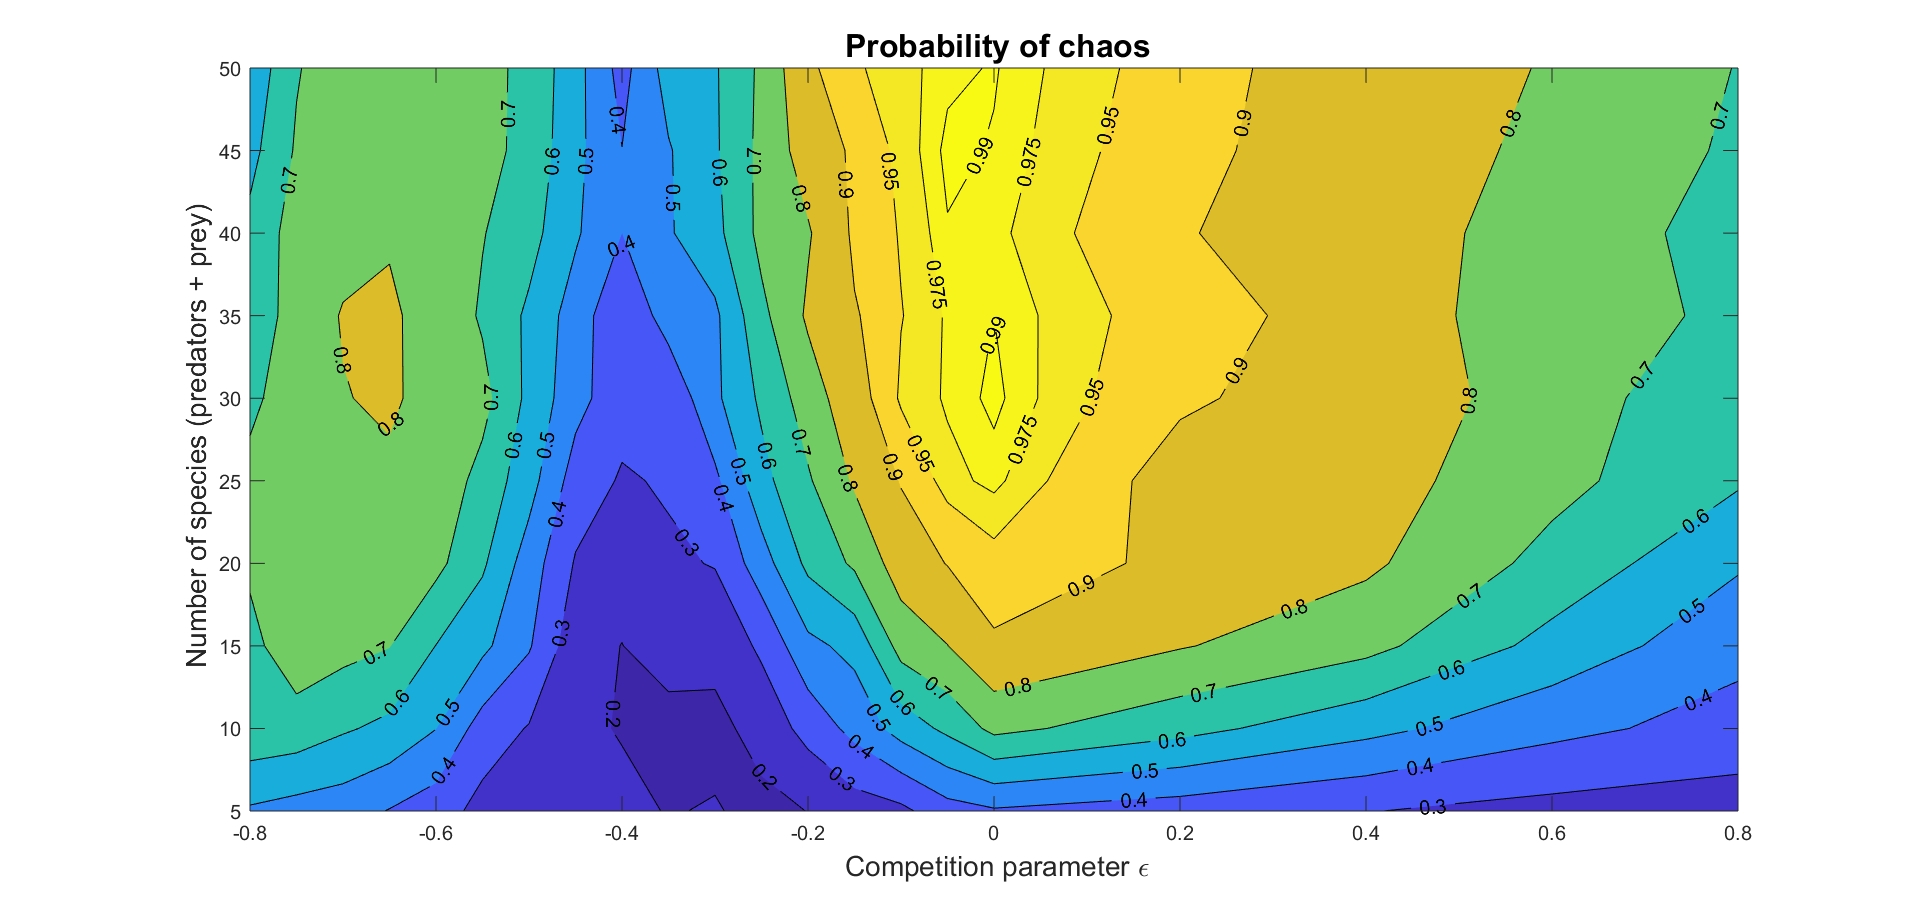
\includegraphics[width=1\columnwidth]{contour.png}
	\end{center}
	\caption{Contour map showing the probability of chaos for various competition parameters (horizontal axis) and number of species (vertical axis). The consumers' population is fixed as $ 2/3 $ of the prey's population. Notice that chaotic attractors appear more easily (i.e., for smaller systems) the closer is the competition to neutral (i.e., $ \epsilon = 0 $).}
	\label{fig:Contour}
\end{figure}

% Biodiversity
Our biodiversity measurements (see figure \ref{fig:Biodiversity}) illustrate several additional effects. In panel C we see that the prey biodiversity is very close to its maximum around the neutral-on-average situation. Also, a maximum is observed for strong intraspecific competition. In panels B and C, we see that the dynamic regime has an influence in the prey biodiversity. Particularly, the average prey biodiversity for ecosystems with stable dynamics is always lower than for cyclic ones, and both of them are lower than for those with chaotic dynamics. Despite the dispersion of our box and whisker plot is high, this conclusion remains true for food webs of different sizes (see figure \ref{fig:BiodBoxAndWhisker} in the Online Appendix). From panel D, we see that the prey biomass remains relatively stable for the whole range of competition parameters, with the exception of strong intraspecific competition, where it reaches a maximum. The predator biomass grows almost linearly as the competition moves leftwards, from neutral-on-average to strong intraspecific, while the prey biomass remains constant. This effect is known from $ 2 $ species systems with Type II saturation functions. 

\begin{figure}
	\begin{center}
		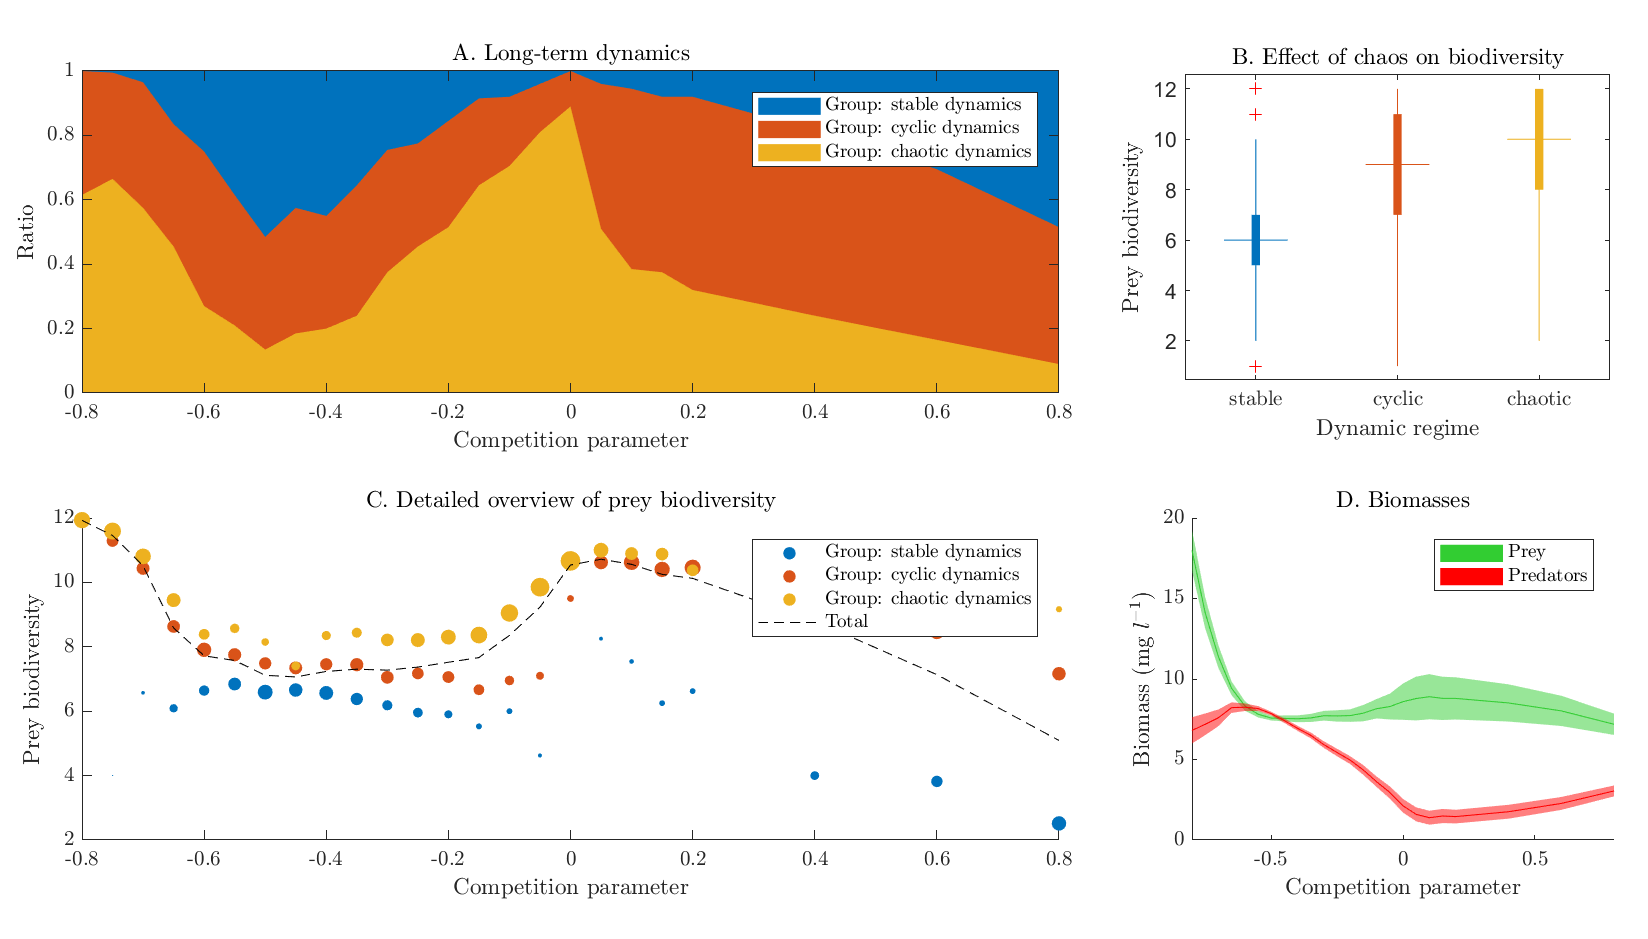
\includegraphics[width=1\columnwidth]{best.png}
	\end{center}
	\caption{Results for a food web with $8$ predator and $12$ prey species. Food webs of different sizes show similar results (see \ref{subsec:ExtraFigures} in Online Appendix). For each value of the competition parameter, $\numReps$ randomly drawn ecosystems were simulated and classified as regular, cyclic or chaotic. Additionally, the number of non-extinct prey species after a stabilization run was registered. \textbf{Panel A}. Ratio of each dynamic regime vs. competition parameter. \textbf{Panel B}. Biodiversity vs. asymptotic regime. Box and whisker plot of the average number of non-extinct prey species grouped by asymptotic regime. \textbf{Panel C}. Average prey biodiversity vs. competition parameter. The dashed line shows the average number of non-extinct prey species grouped by competition parameter. The colored circles represent the average prey biodiversity of the simulations, additionally grouped by dynamical regime (stable, cyclic and chaotic). The relative size of the circles represents the ratio of simulations that led to regular or chaotic dynamics. \textbf{Panel D}. Average biomasses grouped by trophic level vs. competition parameter. The width represents standard deviation.}
	\label{fig:Biodiversity}
\end{figure}